\documentclass[final, 12pt]{beamer}
\usepackage[utf8]{inputenc}
\usepackage[orientation=portrait, size=a1, scale=1.5]{beamerposter}
\usenavigationsymbolstemplate{\beamertemplatenavigationsymbolsempty}

\usepackage{tikz}
\usetikzlibrary{positioning}

% set widths
\newlength{\colwidth}
\setlength{\colwidth}{0.435\paperwidth}

% fonts
\setbeamercolor{block title}{fg=black,bg=white}
\setbeamercolor{block body}{fg=black,bg=white}
\setbeamercolor{item}{fg=black}
\setbeamerfont{caption}{size=\normalsize, series=\bfseries}
\renewcommand{\figurename}{\color{black}{Figure}}

% block style
\setbeamertemplate{block begin}
{
  \par\vskip\medskipamount
  \vskip0.8cm
  \begin{beamercolorbox}[colsep*=0.5ex,dp={2ex},center]{block title}
     \vskip-1cm
    \usebeamerfont{block title}\Large\insertblocktitle
  \end{beamercolorbox}
  {\parskip0pt\par}
  \ifbeamercolorempty[bg]{block title}
  {}
  {\ifbeamercolorempty[bg]{block body}{}{\nointerlineskip\vskip-0.5pt}}
  \vskip0.5cm
  \usebeamerfont{block body}
  \vskip-0.5cm
  \begin{beamercolorbox}[colsep*=0ex,vmode]{block body}
}
\setbeamertemplate{block end}
{
  \end{beamercolorbox}
  \vskip\smallskipamount
}

% title section
\title{Genealogies of Sequential Monte Carlo Algorithms}
\author{Suzie Brown}
\institute{Department of Statistics, University of Warwick}
\logo{
\includegraphics[scale=1.8]{oxwasp3.png}}
\date{}


\begin{document}
\begin{frame}

\vspace*{-35pt}

\centering
\makebox[\textwidth]{
\includegraphics[width=\paperwidth]{warwickhead2.png}}

\vspace*{-160pt}

\huge{\inserttitle}\\[2pt]
\Large{\insertauthor}\\[7pt]
\large{supervised by Jere Koskela, Adam Johansen, Paul Jenkins and Dario Span\`o}\\[7pt]
\normalsize{\insertinstitute}\\[25pt]
\hrule

\vspace*{15pt}

\begin{columns}
\begin{column}{\colwidth}
\begin{block}{Sequential Monte Carlo}

%%% find a generic reference for the following %%%
%%% remove some words %%%
%%% change spacing as required once content is finalised %%%
Suppose we have a hidden Markov model with noisy observations $Y_{1:T}$ of unobservable states $X_{1:T}$.

\begin{center}
\resizebox{0.5\colwidth}{!}{%
\begin{tikzpicture}
\node (yt) {$Y_t$};
\node (thet) [below=of yt] {$X_t$};
\node (yt1) [left=of yt] {$Y_{t-1}$};
\node (thet1) [below=of yt1] {$X_{t-1}$};
\node (dot1) [left=of thet1] {$\dots$};
\node (dot2) [right=of thet] {$\dots$};
\draw[->](thet.north)--(yt.south) node[midway, right] {\footnotesize{$g$}};
\draw[->](thet1.north)--(yt1.south) node[midway, right] {\footnotesize{$g$}};
\draw[->](thet1.east)--(thet.west) node[midway, above] {\footnotesize{$f$}};
\draw[->](dot1.east)--(thet1.west) node[midway, above] {\footnotesize{$f$}};
\draw[->](thet.east)--(dot2.west) node[midway, above] {\footnotesize{$f$}};
\end{tikzpicture}
}
\end{center}
\vspace*{-20pt}

We may want to infer filtering distributions $p(x_t | y_{1:t})$, or smoothing distributions $p(x_{1:t} | y_{1:t})$. 
These are not available analytically, except in linear Gaussian models. \\[12pt]

SMC [1] approximates the posterior distributions by sampling $N$ particles from the prior distribution and iterating the following steps:
\begin{enumerate}
\item \textbf{Propagate:} move particles according to the Markov kernel $f$
\item \textbf{Calculate weights:} weight particles according to how likely they are to produce the observations through $g$
\item \textbf{Resample:} duplicate high-weight particles and kill off low-weight particles to obtain a new sample of size $N$.
\end{enumerate}

\vspace*{10pt}

The figure shows how the population of particles looks at each step, before resampling. The purple ribbon shows the exact posterior mode and 95\% credible interval.
\begin{figure}
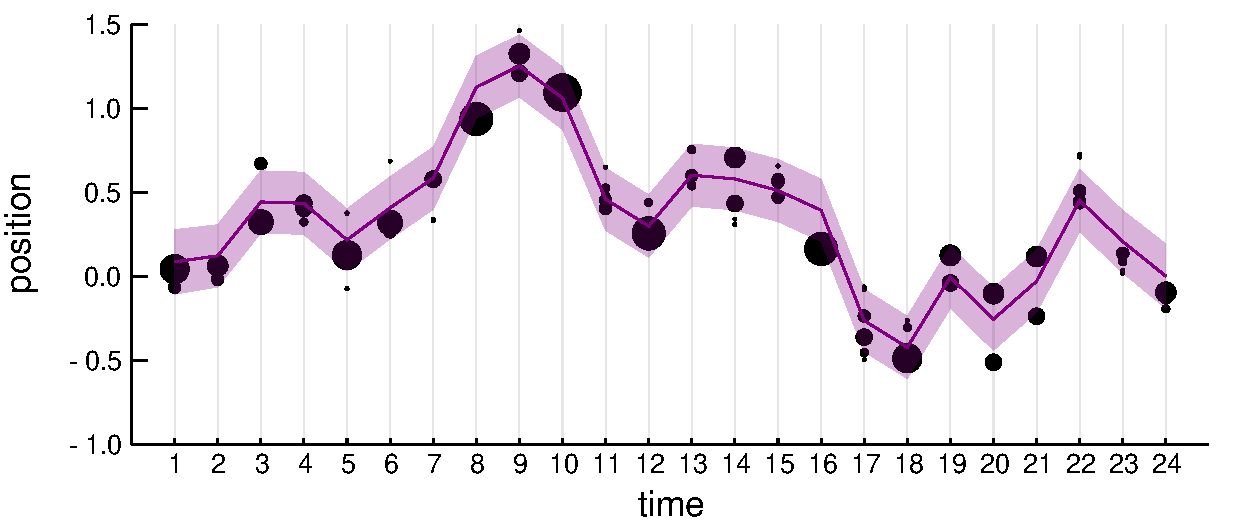
\includegraphics[width=\colwidth]{smc_kalman_3.pdf}
\caption{Exact posterior (purple) and weighted SMC particles before resampling (black) for a linear Gaussian model.}
\end{figure}
\end{block}

\begin{block}{Ancestral Degeneracy}
However, these particles cannot approximate the smoothing distributions. For that we need a sample of \emph{trajectories} covering all $t$ time steps, not just a sample of particles at each time step.\\[10pt]

We have a sample of $N$ such trajectories: the ancestral trajectories of each of the $N$ particles alive at time $t$.
But due to the resampling mechanism, these ancestries coalesce backwards in time, leaving many fewer than $N$ distinct samples at time 0. 

\begin{figure} %%% remake this plot with a less weird realisation? %%%
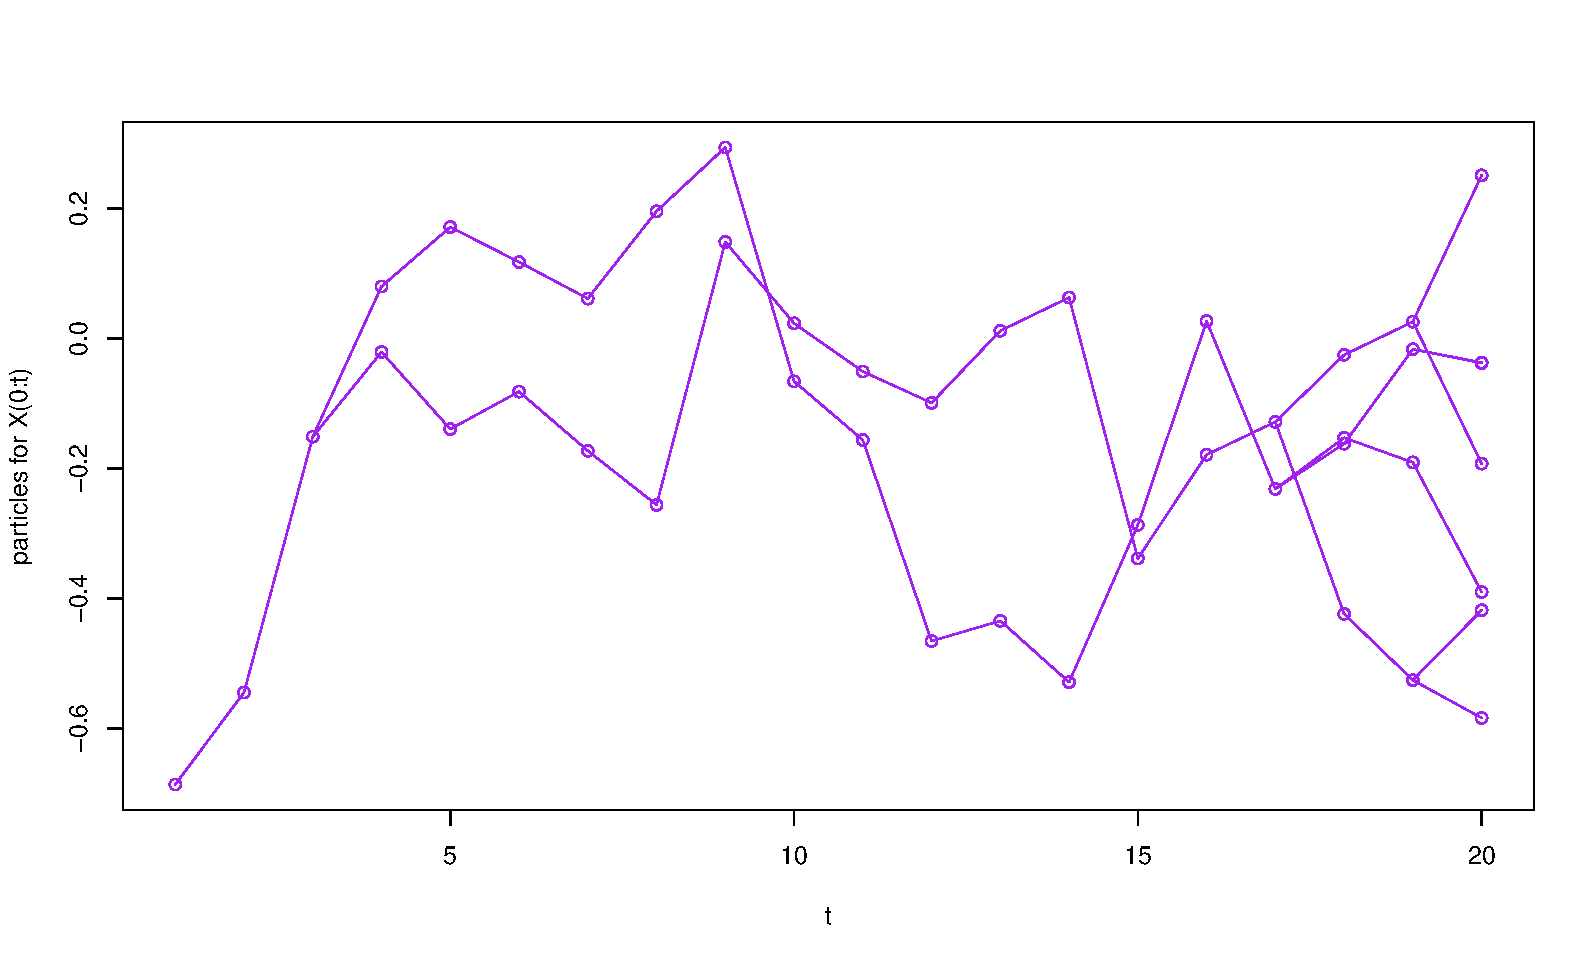
\includegraphics[width=0.9\colwidth]{degeneracy.pdf}
\caption{Trajectories from a sample of N=6 particles. For most of the time there are just one or two distinct lineages.}
\end{figure}

This phenomenon is known as \emph{ancestral degeneracy} [1]. It can be mitigated by changing the resampling procedure, but it cannot be eradicated.
\end{block}
\end{column}

\begin{column}{\colwidth}

\vspace*{-80pt}

\begin{block}{The Kingman Coalescent}
The Kingman coalescent [2] is a continuous-time process which describes the asymptotic genealogies of many population models.\\[10pt]

The process starts with a population of size $N$ and ends when all of the lineages have merged into one.
Each pair of lineages merges with rate 1, meaning that the total merger rate is higher when there are more distinct lineages. 
\begin{figure}
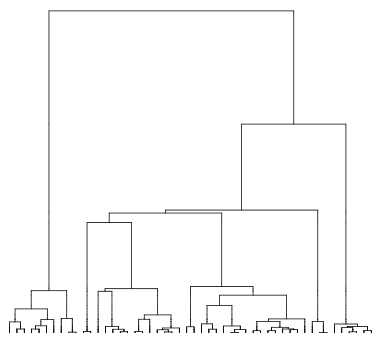
\includegraphics[width=0.8\colwidth]{kingman.png}
\caption{A realisation of the Kingman coalescent for a population of size N=50. \textmd{(Source: Wikimedia Commons)}}
\end{figure}
The resulting coalescent has many lineages for only a short time, and spends most of its time with just two or three distinct lineages.
\end{block}

\vspace*{15pt}

\begin{block}{Asymptotic SMC Genealogies}
The rate of coalescence of SMC genealogies depends on the resampling scheme used. 
Schemes giving higher variance offspring numbers produce faster coalescence.\\[10pt]

To obtain convergence to the Kingman coalescent, which has rate 1, we rescale time by the inverse coalescence rate, and consider the asymptotic regime as  $N\to\infty$.\\[10pt]

Convergence to the Kingman coalescent is only proved for the simple case of multinomial resampling [3]. We have since extended this result to cover conditional SMC with multinomial resampling.\\[10pt]

Next we would like to analyse the coalescents induced by alternative resampling schemes such as residual and stratified resampling. These schemes reduce the offspring variance and hence the coalescence rate, and are more popular among practitioners.
\end{block}

\vspace*{50pt}

\hrule
\begin{block}{References}
\begin{enumerate}
\item Doucet, A., \& Johansen, A. M. (2009). A tutorial on particle filtering and smoothing: Fifteen years later. \textit{Handbook of nonlinear filtering}, 12(656-704), 3.
\item Kingman, J.F.C. (1982). The coalescent. \textit{Stochastic processes and their applications}, 13(3), pp.235-248.
\item Koskela, J. et al. (2018).  Asymptotic genealogies of interacting particle systems with an application to sequential Monte Carlo. \textit{arXiv preprint} arXiv:1804.01811.
\end{enumerate}
\end{block}

\end{column}
\end{columns}

\end{frame}
\end{document}